%---------------------------------------------------------------------------%
%->> Section 3.2: 传播感知的多模态故障指纹构建方法
%---------------------------------------------------------------------------%

\section{传播感知的多模态故障指纹构建方法}

ASE 2024 的 FAIL 研究对 2010 年至 2022 年间公开报道的 2457 起软件故障进行了统计，结果表明，其中 85\% 属于重复或相似场景，77\% 会在同一组织内再次出现，53\% 会在不同组织间重复出现\cite{fail-anandayuvaraj2024}。这说明，生产环境中的大量故障并不是孤立事件。历史故障中留下的观测模式和诊断线索，具有直接复用的价值。

然而，在实际运维场景中，历史诊断案例的诊断经验往往难以被直接复用。其核心问题在于，当前故障与历史故障之间缺乏统一的表征框架。现有做法常用工单标题、案例摘要或人工标注的故障类型描述故障，例如“服务超时”，“数据库异常”，“调用链抖动”等。这类描述便于归档，却往往停留在症状层面，难以回答更关键的问题：异常首先出现在哪里、指标如何变化、日志呈现出何种模式，以及异常沿何种依赖关系传播。以“服务超时”为例，它既可能由数据库连接池耗尽引起，也可能源于缓存雪崩或网络抖动；与此同时，不同根因也可能表现出相近的外部症状。这种现象表明，真正具备跨场景复用价值的，并非粗粒度的静态标签，而是故障发生时多模态观测数据所蕴含的细粒度故障模式。

要把这些模式表征出来，难点在于相关线索分散在指标、日志和调用链路中。三类数据的结构、语义层级和特征形式差异很大，不能直接比较。为了使历史诊断经验能够被稳定召回，系统需要为一次故障构建一种同时保留多模态观测特征与传播信息、且便于跨实例比较的统一表示。为此，本文提出故障指纹（Fault Fingerprint）的概念，用固定维度向量表示一次故障窗口内的多模态观测，并以向量距离衡量故障之间的相似性。在此基础上，本文提出传播感知的多模态故障指纹构建方法（Propagation-Aware Multimodal Fault Fingerprinting，PMF）。该方法首先对指标、日志和调用链路进行统一表示；随后围绕故障传播过程提取多模态特征；最后通过标准化与特征筛选生成故障指纹。

\subsection{故障指纹构建方法的设计}

故障指纹主要用于相似故障实例的检索。它的核心目标不是为故障‘贴标签分类’，而是对比当前现象与历史记录在故障演化过程上的相似度。因此，构建故障指纹时需要把握好特征的平衡：既要精准提取出故障形成与传播的核心规律，又要剔除掉特定场景下的偶然干扰（如具体的服务实例名或环境参数），确保提取出的特征具有足够的通用性和跨场景匹配能力。

\begin{figure}[tbp]
    \centering
    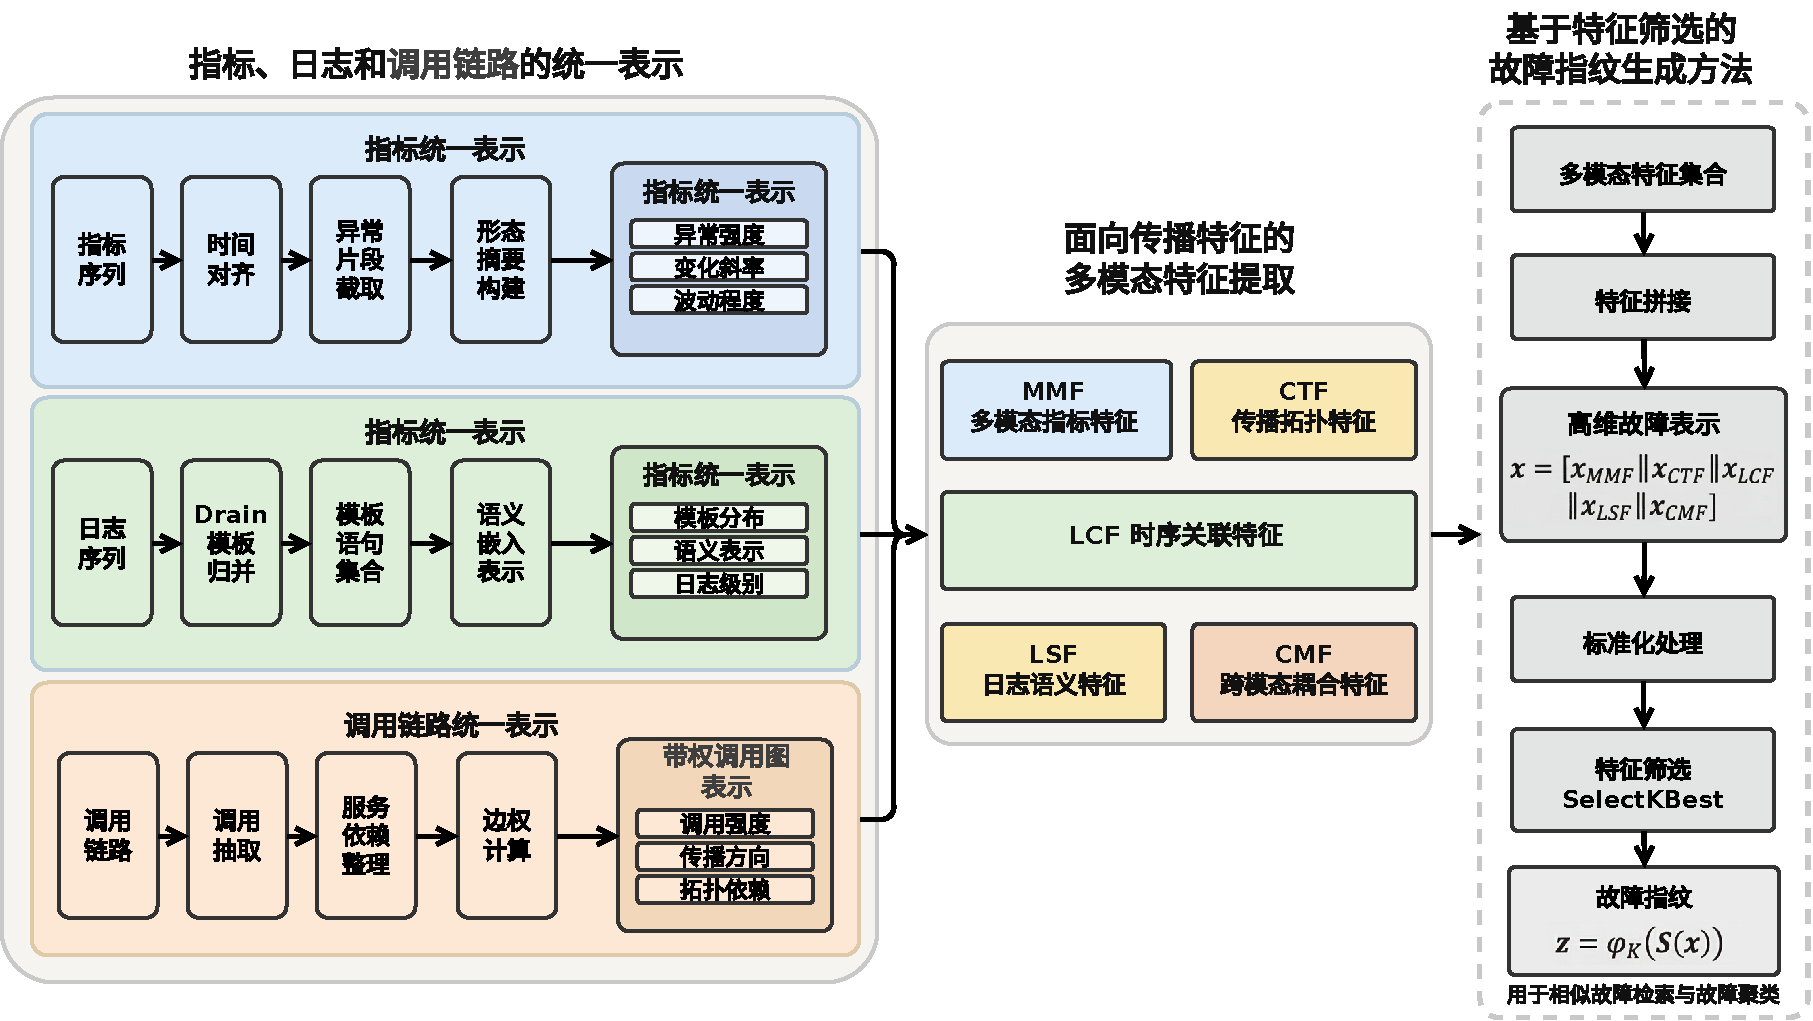
\includegraphics[width=\textwidth]{Figures-Src/Chap3-Methodology/fault-representation/chart.pdf}
    \bicaption{\enspace 传播感知的多模态故障指纹构建流程}{\enspace Pipeline of Propagation-Aware Multimodal Fault Fingerprinting}
    \label{fig:fingerprint_framework}
\end{figure}

图\ref{fig:fingerprint_framework}给出了传播感知的多模态故障指纹构建方法的整体三阶段构建流程。

\begin{enumerate}[label=（\arabic*）]

    \item \textbf{指标、日志和调用链路的统一表示。}  该阶段以故障窗口内的原始指标、日志和服务调用链路为输入，分别形成指标形态摘要、日志模板语义表示和带权服务调用图三类中间表示。其目的不是直接生成故障指纹，而是先将结构、粒度和语义层级不同的观测数据转换为可比较的表示，为后续统一建模提供基础。

    \item \textbf{面向故障传播特征的多模态特征提取。}  该阶段以上一步得到的三类中间表示为输入，进一步提取多模态指标特征、传播拓扑特征、时序关联特征、日志语义特征和跨模态耦合特征。其作用是在统一表示基础上，保留真正与故障传播过程相关的信息，使故障表示不仅反映局部异常，还能够体现传播路径、上下游影响和跨模态联动关系。

    \item \textbf{基于特征筛选的故障指纹生成方法。}  该阶段以高维多模态特征为输入，通过标准化与特征筛选生成固定维度的故障指纹。其作用是从大量候选特征中保留更具稳定性和区分能力的部分，使最终表示既能保留故障传播特征，又适合用于相似故障检索与历史经验绑定。
\end{enumerate}

以下示例有助于进一步理解设计要点。\textit{某电商系统在不同时间发生的两次支付超时故障。第一次故障由数据库连接池耗尽引起，表现为数据库连接错误日志出现、支付服务响应时延持续升高，并进一步导致上游订单服务超时；第二次故障由缓存服务宕机引起，表现为缓存不可用、数据库查询压力激增以及支付服务时延上升}。两次故障在入口症状上都表现为“支付超时”，但其内部形成过程并不相同。若仅依赖工单标题或故障标签，系统很容易将二者归为同一类故障，进而匹配到并不合适的历史排查经验。相反，若故障表示能够同时保留日志线索、指标变化和传播路径，那么这两次故障在表示空间中应当具有可区分性。

基于这一考虑，本文将\textbf{故障指纹}定义为：在故障窗口期内，从指标、日志和服务调用拓扑中提取的、用于相似故障检索的固定维度嵌入向量。若两个故障事件在故障指纹空间中的距离较近，则表明二者在微服务上下文、观测模式和传播特征上更为相似，因而更可能对应相同或相近的故障形成过程；若距离较远，则说明其内部模式存在较大差异。

本文将一次故障定义为一个故障事件，表示为
\begin{equation}
\mathcal{E}=\langle \mathcal{M}, \mathcal{L}, \mathcal{G}\rangle
\end{equation}
其中，$\mathcal{M}$ 表示故障窗口期内的指标集合，$\mathcal{L}$ 表示日志集合，$\mathcal{G}$ 表示服务调用拓扑。故障指纹构建即是定义映射函数
\begin{equation}
\mathbf{z}=F(\mathcal{E}), \quad \mathbf{z}\in\mathbb{R}^{K}
\end{equation}
其中，$\mathbf{z}$ 表示故障事件 $\mathcal{E}$ 对应的故障指纹。

对于任意两个故障事件 $\mathcal{E}_i$ 与 $\mathcal{E}_j$，理想情况下，若二者对应相同或相近的故障，则其故障指纹表示应更接近；若二者的故障形成过程存在显著差异，则其故障指纹表示应保持分离性。为了使映射 $F$ 满足这一要求，本文对故障指纹构建提出如下两点设计要求：

\begin{itemize}
    \item \textbf{稳定性。} 即指纹的提取必须过滤掉特定服务实例名、环境参数或局部瞬时波动的干扰，确保相同成因的故障在不同的请求、实例和流量背景下，仍能稳定映射为相近的表示；
    
    \item \textbf{可区分性。} 即指纹不能仅停留在粗粒度的表面症状层面，而应深入保留故障演变与传播的关键线索，从而能够准确区分那些“入口症状相近但内部成因完全不同”的故障。
\end{itemize}

故障指纹构建映射 $F$涉及可观测数据的统一表征、面向传播特征的多模态特征提取和基于特征筛选的故障指纹生成，下面分别进行详细阐述。

\subsection{指标、日志和调用链路的统一表示}

故障窗口内的原始观测包括指标、日志和调用链路数据。三类数据在表示形式和统计特征上差异很大：指标是连续采样的时间序列，日志是包含大量变量和上下文的离散文本流，调用链路则体现为服务之间的调用关系及其结构依赖。如果直接将它们拼接到一起，不仅会带入大量与故障特征无关的实例级细节，也难以建立跨故障稳定比较的基础。因此，本文先分别对三类观测进行统一表示，得到三类中间表示，为后续特征提取提供输入。

\textbf{指标形态摘要。}
对指标数据而言，关键并不是保留完整时间序列，而是抓住故障期间的变化形态。为此，本文以“服务$\times$指标”二元组为基本统计单元，在故障窗口内完成时间对齐，并提取异常强度、变化斜率、跃迁幅度、波动性和尖峰比例等统计量。用于比较的并不是某一时刻的精确取值，而是故障期间是否出现了持续升高、快速跃迁、剧烈波动或尖峰突发等模式。例如，数据库连接池耗尽通常表现为连接数持续升高并逼近上限，网络抖动则更常表现为时延的明显波动。经过这一步，原始指标序列被压缩为相对稳定的形态摘要，从而减弱负载波动、采样频率差异和局部瞬时扰动对比较结果的影响。

\textbf{日志模板与语义表示。}
日志数据的难点主要在于表面表达离散，而且容易受到实例变量干扰。相同故障在不同实例中留下的日志往往语义相近，但文本形式并不相同，例如“Connection timeout to DB instance db-01”和“Connection timeout to DB instance db-02”。为此，本文首先采用 He 等提出的 Drain 在线日志解析算法~\cite{drain-he2018}，将原始日志归并为模板序列。Drain 通过固定深度的解析树，将日志文本中的变量部分替换为通配符，从而将上述两条日志统一归并为模板“Connection timeout to DB instance <*>”。

在模板归并之后，本文进一步采用预训练语义嵌入模型对模板文本进行编码：
\begin{equation}
\mathbf{e}_k = f_{\text{emb}}(T_k)
\end{equation}
其中，$T_k$ 表示日志模板，$\mathbf{e}_k$ 表示对应的模板语义向量。这样做的目的，是将语义相近但表面表述不同的日志模式映射到更为接近的语义空间区域。例如，“Connection timeout”和“Database connection failed”虽然文本不同，但在语义空间中的距离较近，因此可以被识别为相近的错误模式。如图\ref{fig:drain_parsing}所示，原始日志在解析树中按层次逐步匹配，并最终归并至相应模板，从而将实例标识、请求编号和变量取值等高频变化项从日志主体中分离出来。经过这一处理后，日志观测被转换为更适合跨故障比较的日志模板及其语义表示。

\begin{figure}[tbp]
    \centering
    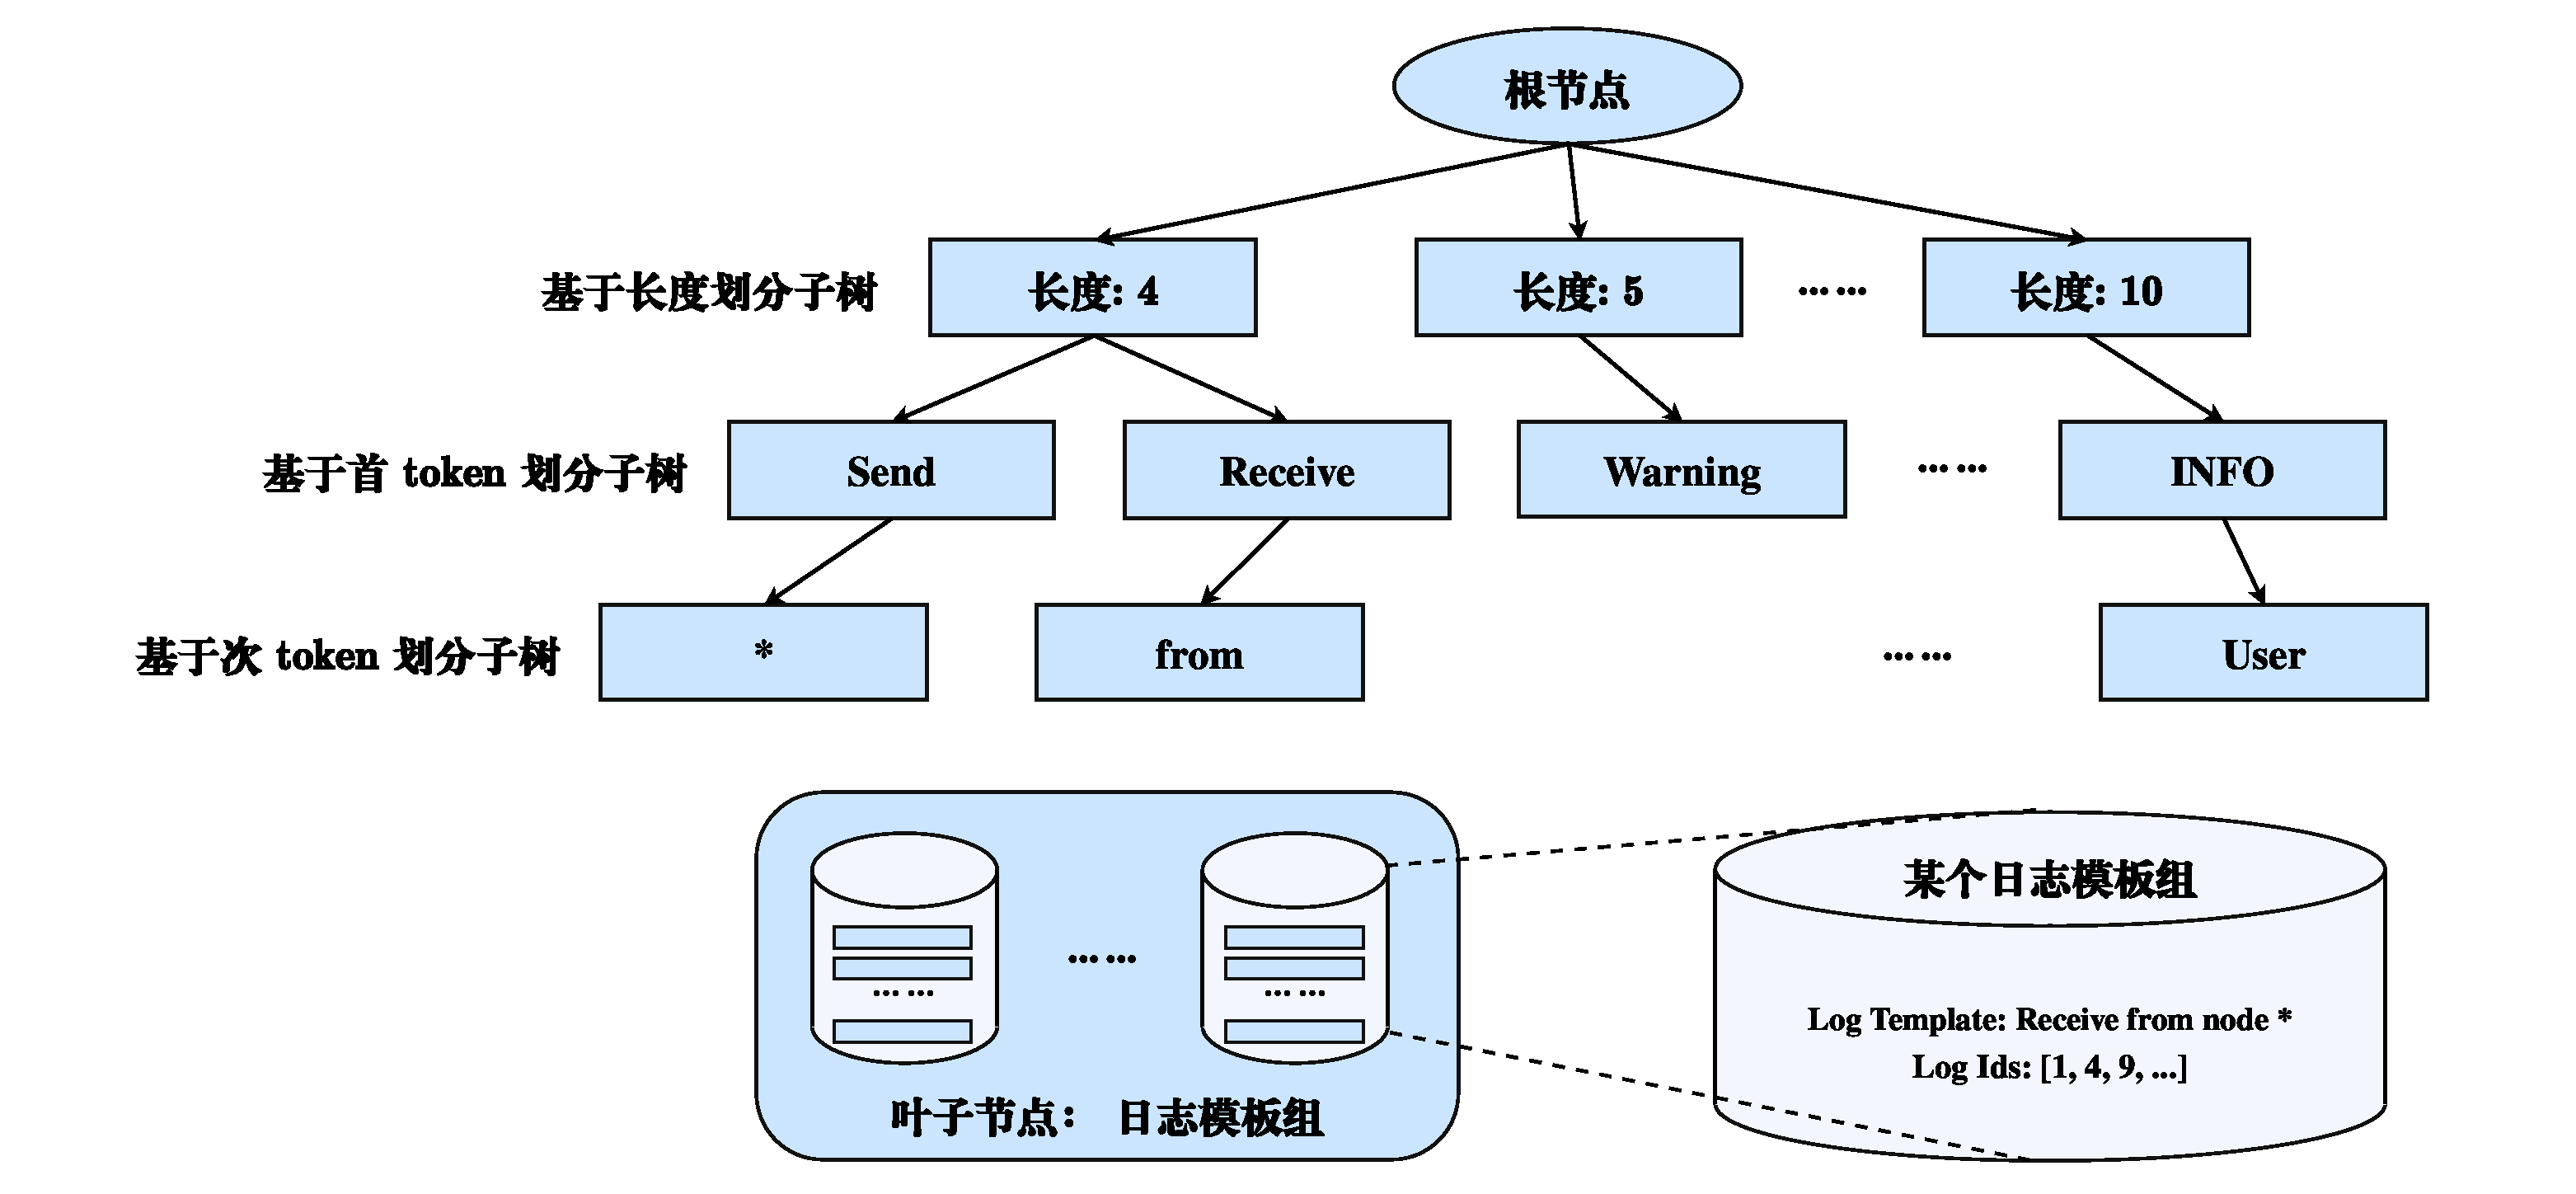
\includegraphics[width=0.9\textwidth]{Figures-Src/Chap3-Methodology/drain/chart.pdf}
    \bicaption{\enspace Drain日志模板解析与模板归并}{\enspace Drain-based Log Template Parsing and Template Grouping}
    \label{fig:drain_parsing}
\end{figure}

\textbf{带权服务调用图。}
调用链路部分保留的是故障的结构上下文。微服务故障通常不会停留在某一个服务内部，而会沿着服务依赖关系向上下游传播。例如，数据库连接池耗尽可能先导致数据访问层服务响应变慢，继而引发业务逻辑层服务超时，最终传播到前端 API 服务。不同故障之间的差异，不仅体现在哪些服务出现异常，还体现在异常沿哪条依赖链演化、哪些节点处于关键传播位置，以及上下游耦合强度如何变化。为此，本文从调用链路数据中提取服务间调用边，构建服务级调用图 $G=(V,E)$，并以故障窗口内的调用计数$c_{i,j}$作为边$(i,j)$ 的原始权重。其中，节点表示服务实体，边的原始权重反映服务之间的调用频次。该有向图及其原始边权共同保留了传播方向和耦合强度，并为后续多模态特征提取提供统一输入。在后续传播拓扑特征提取阶段，本文再基于这些原始边权进行归一化处理，并计算传播相关统计量。

经过上述处理，原始指标、日志和调用链路分别被表示为指标形态摘要、日志模板及其语义表示，以及带权服务调用图。这些中间表示构成了后续传播特征提取的输入。

\subsection{面向传播特征的多模态特征提取}

统一表示之后，跨故障比较的基础已经建立，但最终检索效果仍取决于所保留特征是否真正与故障传播过程相关。若直接将三类中间表示拼接，虽然能够保留部分信息，但仍然难以突出传播路径、时序联动和跨模态协同等关键因素。为此，本文围绕指标异常、传播结构、时序关系、日志语义和跨模态耦合提取五类特征。考虑到服务组合、调用边和日志模板数量较多，本文对高频项直接保留其统计特征，对低频组合采用固定维度哈希编码，以避免特征维度随系统规模增长而持续膨胀。

\textbf{指标形态特征（Metric Morphology Features，MMF）。}
MMF 是故障指纹中描述指标模态异常形态的特征分量。本文首先统计高频服务和高频指标的异常强度分布，再对每个”服务$\times$指标”组合计算平均强度、变化斜率、跃迁幅度、波动性和尖峰比例。对于出现次数较少的服务--指标组合，则采用固定维度哈希编码保留其异常信息。该类特征主要用于区分资源持续升高、局部性能抖动和短时突发波动等不同类型的指标异常。

\textbf{传播拓扑特征（CTF）。}
CTF 用于刻画异常在服务依赖结构中的传播组织方式。微服务故障通常不会停留在单一服务内部，而会沿上下游依赖关系扩散。因此，异常扩散涉及哪些边、哪些节点处于传播中心、哪些区域承载更高扩散风险，都应作为故障表示的重要组成部分。设故障窗口内调用边 $(i,j)$ 的调用计数为 $c_{ij}$，则其归一化权重记为
\begin{equation}
a_{ij}=
\begin{cases}
\dfrac{c_{ij}}{\sum_{(p,q)\in E} c_{pq}}, & (i,j)\in E \\
0, & \text{otherwise}
\end{cases}
\end{equation}
在此基础上，分别计算节点的入度 $d_i^{\text{in}}$ 与出度 $d_i^{\text{out}}$，并定义拓扑中心性与传播倾向：
\begin{equation}
c_i^{\text{topo}} = d_i^{\text{in}} + d_i^{\text{out}}
\end{equation}
\begin{equation}
p_i^{\text{prop}} = \frac{d_i^{\text{out}}}{d_i^{\text{in}} + d_i^{\text{out}} + \epsilon}
\end{equation}
其中，拓扑中心性反映服务在传播结构中的连接程度，传播倾向衡量异常继续向下游扩散的可能性。为了进一步估计异常在整张调用图上的传播范围，本文使用带权随机游走计算故障传播影响力，并针对微服务故障传播的连续带权特性做三项调整。若服务 $i$ 对应节点 $v_i$，则节点影响力初始化不采用均匀分布，而是由节点上的故障严重程度决定：
\begin{equation}
r_i^{(0)} = \frac{\text{severity}(v_i)}{\sum_{v_j \in V} \text{severity}(v_j)}
\end{equation}
转移概率由调用边权重定义：
\begin{equation}
W_{ij} = \frac{c_{ij}}{\sum_{k \in \text{out}(i)} c_{ik}}
\end{equation}
同时，引入时间衰减因子刻画传播时序性：
\begin{equation}
\mathbf{r}^{(t+1)} = (1-\alpha) \mathbf{W}^{\top}(\mathbf{r}^{(t)} \odot \boldsymbol{\beta}^{\Delta t}) + \frac{\alpha}{|V|}\mathbf{1}
\end{equation}
其中，$\mathbf{W}$ 为按出边归一化后的带权转移矩阵，$\alpha$ 为阻尼系数，$\boldsymbol{\beta}^{\Delta t}$ 为时间衰减因子向量，$\odot$ 表示逐元素乘法，$\mathbf{r}$ 为服务影响力向量。经过上述处理，CTF 由边频次统计、入出度分布、全局结构统计、拓扑中心性、传播倾向和传播影响力共同构成，用于描述故障围绕哪些关键节点展开，以及异常可能沿哪些依赖链继续扩散。

\textbf{时序关联特征（LCF）。}
LCF 用于区分“结构上可能传播”和“运行时确实联动”这两种不同情形。静态调用链路只能说明服务之间存在传播路径，并不能证明故障在当前窗口内真的沿该路径扩散。为此，本文在服务级别对指标信号与日志信号进行分钟级聚合，并在有限滞后窗口内搜索最优相关性：
\begin{equation}
\rho_i = \max_{\ell \in [-L,L]} \left|\operatorname{corr}\left(m_i(t), l_i(t+\ell)\right)\right|
\end{equation}
其中，$m_i(t)$ 表示服务 $i$ 的指标信号，$l_i(t)$ 表示服务 $i$ 的日志信号，$\ell$ 表示滞后步长。除最优相关性外，本文还保留最优滞后位置、滞后直方图和整体统计结果，用于描述不同服务中“指标异常领先日志”或“日志异常领先指标”的时序关系。LCF 为拓扑上的潜在传播关系补充了时间证据，从而避免仅凭结构邻接关系误判真实传播链。

\textbf{日志语义特征（Log Semantic Features，LSF）。}
LSF 用于从模板分布和时间强度两个方面刻画日志异常，其处理对象为故障窗口内经 Drain 解析后得到的日志模板序列。具体而言，系统统计各模板的出现频次及分布，提取 ERROR、WARN、INFO 各级别日志的占比，并计算故障窗口内的日志突发强度（单位时间内的异常等级日志数量）。由于统一表示阶段已经引入模板语义嵌入，不同文本表达但语义相近的模板能够在统一语义空间中对齐，因此 LSF 同时保留模板频次及语义归一化后的统计结果，使日志异常模式在跨故障比较中具有语义一致性。

\textbf{跨模态耦合特征（Cross-Modal Coupling Features，CMF）。}
CMF 用于刻画指标、日志和调用链路之间的联动关系，其基本假设是真实故障往往在多个模态中同时留下异常信号。在指标—日志联动层面，系统计算服务粒度上指标异常出现时间与日志异常出现时间的时差分布；在链路—日志联动层面，统计调用边上时延升高事件与下游异常日志事件的共现比例。此外，CMF 综合统计服务数、指标种类数、日志量、上下游服务规模、平均边权、异常强度和日志错误比例等全局规模变量，并进一步计算传播风险分数，以反映异常规模、传播范围与日志响应强度是否呈现一致增强，从而区分真实多模态联动故障与单模态假阳性事件。

基于上述三类中间表示，本文提取了 MMF、CTF、LCF、LSF 和 CMF 五类特征。MMF 描述故障在指标层面的异常形态，CTF 和 LCF 刻画传播结构及其时序证据，LSF 提供日志层面的补充信息，CMF 反映不同模态之间是否存在一致的异常增强现象。这五类特征共同构成后续故障指纹生成的输入。

\subsection{基于特征筛选的故障指纹生成方法}

经过统一表示与传播特征提取两个阶段后，一次微服务故障已经被表示为五类面向传播特征的高维特征。但这些特征还不能直接作为最终故障指纹用于相似故障检索，因为不同特征块在数值范围、稀疏程度和统计稳定性上存在明显差异。例如，指标特征通常表现为连续数值，日志特征则往往是高度稀疏的计数；同时，也存在部分特征维度在不同故障之间缺乏足够区分能力。若将所有特征不加选择地保留到最终表示中，故障指纹将包含较多冗余特征和弱相关特征，从而削弱相似故障在表示空间中的聚合效果。

为此，本文首先将五类特征拼接为统一的高维故障表示：
\begin{equation}
\mathbf{x} =
\left[
\mathbf{x}^{\text{MMF}} \,\Vert\,
\mathbf{x}^{\text{CTF}} \,\Vert\,
\mathbf{x}^{\text{LCF}} \,\Vert\,
\mathbf{x}^{\text{LSF}} \,\Vert\,
\mathbf{x}^{\text{CMF}}
\right]
\end{equation}
其中，$\Vert$ 表示向量拼接操作。由于不同特征块在量纲和分布上存在显著差异，本文先对拼接后的特征向量进行标准化处理，以减弱数值范围差异对后续判别过程的影响。

在此基础上，为保留对故障区分更有贡献的特征，本文采用单变量方差分析的 \texttt{SelectKBest} 方法对高维特征进行筛选~\cite{scikit-learn,scipy}，记筛选映射为 $\phi_K(\cdot)$。最终故障指纹定义为
\begin{equation}
\mathbf{z} = \phi_K(\tilde{\mathbf{x}})
\end{equation}
其中，$\tilde{\mathbf{x}}$ 表示标准化后的高维特征向量，$\mathbf{z}$ 表示筛选后的故障指纹。通过该步骤，最终表示在保留多模态关键信息的同时，减少了低价值维度的干扰，从而提高故障指纹的判别性与检索稳定性。


\makeatletter
\@addtoreset{algorithm}{chapter}
\setlength{\@fptop}{0pt}
\makeatother
\renewcommand{\thealgorithm}{\thechapter-\arabic{algorithm}}
\floatname{algorithm}{算法}

\algrenewcommand\algorithmicrequire{\textbf{输入：}}
\algrenewcommand\algorithmicensure{\textbf{输出：}}
\algrenewcommand\algorithmicforall{\textbf{对每个}}
\algrenewcommand\algorithmicdo{\textbf{执行}}
\algrenewcommand\algorithmiccomment[1]{\hfill// #1}
\algtext*{EndFor}

\begin{algorithm}[!t]
    \caption{\enspace PMF 故障指纹构建算法}
    \label{alg:fault_fingerprint}
    \begin{algorithmic}[1]
        \Require 训练故障集 $\mathcal{D}=\{\mathcal{E}_i\}_{i=1}^{N}$，保留维度 $K$，相关性阈值 $\rho_{\max}$
        \Ensure 故障指纹映射 $F(\cdot)$
        \State InitEncoding($\mathcal{D}$) \Comment{初始化高频统计项与低频组合的哈希编码规则}
        \ForAll{故障事件 $\mathcal{E}_i \in \mathcal{D}$}
            \State $\mathbf{m}_{\mathcal{E}_i} \leftarrow$ BuildMetrics($\mathcal{E}_i$) \Comment{构造指标形态摘要}
            \State $\mathbf{l}_{\mathcal{E}_i} \leftarrow$ BuildLogs($\mathcal{E}_i$) \Comment{构造日志模板及其语义表示}
            \State $G_{\mathcal{E}_i} \leftarrow$ BuildCalls($\mathcal{E}_i$) \Comment{构造服务级调用图}
            \State $(\mathbf{x}^{\mathrm{MMF}}_{\mathcal{E}_i},\mathbf{x}^{\mathrm{CTF}}_{\mathcal{E}_i},\mathbf{x}^{\mathrm{LCF}}_{\mathcal{E}_i},\mathbf{x}^{\mathrm{LSF}}_{\mathcal{E}_i},\mathbf{x}^{\mathrm{CMF}}_{\mathcal{E}_i})$
            \State \hspace{1.5em} $\leftarrow$ ExtractFeatures($\mathbf{m}_{\mathcal{E}_i},\mathbf{l}_{\mathcal{E}_i},G_{\mathcal{E}_i}$) \Comment{提取五类传播特征}
            \State $\mathbf{x}_{\mathcal{E}_i} \leftarrow$ ConcatFeatures$(\mathbf{x}^{\mathrm{MMF}}_{\mathcal{E}_i},\mathbf{x}^{\mathrm{CTF}}_{\mathcal{E}_i},\mathbf{x}^{\mathrm{LCF}}_{\mathcal{E}_i},\mathbf{x}^{\mathrm{LSF}}_{\mathcal{E}_i},\mathbf{x}^{\mathrm{CMF}}_{\mathcal{E}_i})$ \Comment{拼接得到高维故障表示}
        \EndFor
        \State $\mathbf{X} \leftarrow$ StackMatrix$(\{\mathbf{x}_{\mathcal{E}_i}\}_{i=1}^{N})$ \Comment{构造特征矩阵}
        \State $S \leftarrow$ FitNormalizer$(\mathbf{X})$ \Comment{拟合标准化映射}
        \State $\tilde{\mathbf{X}} \leftarrow S(\mathbf{X})$ \Comment{得到标准化特征矩阵}
        \State $\mathbf{s} \leftarrow$ ComputeVarianceScore$(\tilde{\mathbf{X}})$ \Comment{计算各维特征的方差得分}
        \State $\mathcal{S}_{K} \leftarrow$ SelectFeatures$(\mathbf{s},\tilde{\mathbf{X}},K,\rho_{\max})$ \Comment{按得分排序并结合相关性约束保留 $K$ 维特征}
        \State 定义故障指纹映射 $F(\mathcal{E})=\left(S(\mathbf{x}_{\mathcal{E}})\right)_{\mathcal{S}_{K}}$
        \State \Return $F(\cdot)$
    \end{algorithmic}
\end{algorithm}



算法\ref{alg:fault_fingerprint}给出了 PMF 的离线构建过程。该过程首先基于训练故障集完成指标、日志和调用链路的统一表示与传播特征提取，随后通过标准化与特征筛选学习故障指纹映射。该映射可用于后续故障实例的指纹生成，并进一步支持相似故障检索、故障聚类和 SOP 绑定。

